\documentclass[]{article}
\usepackage{lmodern}
\usepackage{amssymb,amsmath}
\usepackage{listings}
\usepackage{graphicx}

\begin{document}

\section{Linear Filters and Frequency Analysis}
\label{linear-filters-and-frequency-analysis}

\subsection{Linear Filtering, Convolution and Impulse Response}
\label{linear-filtering}

Linear filtering is an image processing technique where a filter is applied to
an input image to produce an output. Inputs and outputs of the linear filtering
operation are images. The filter itself can be thought of as an image as well.
The filtering operation corresponds to sliding the filter on the input pixel by
pixel and computing the output. 

The output O(x,y) is given by following equation
\begin{equation}
  O(x,y) = \sum_{x_*=-K}^{K}\sum_{y_*=-K}^{K}{W(x_*,y_*)I(x+x_*,y+y_*)}
\end{equation}
where $W$ is the filter of size $(2K+1)*(2K+1)$, $I$ is the input image and $O$
is the output image. For each position $(x,y)$ the output is given by the
linear correlation of the filter with the sub-area in the same position in the
input image. The output pixel at $(x,y)$ is computed by taking the sum over the
products of the filter values at positions $(x_*,y_*)$ and the input values
centered at $(x,y)$ offset by $(x_*,y_*)$.

Convolution is an operation closely related to linear correlation. The term
convolution might be familiar to people following news on neural networks and
deep learning. We are talking about the convolution in Convolutional Neural
Networks. Convolution is defined as
\begin{equation}
  I_1(x,y) \ast I_2(x,y) = \sum_{x_*=-\infty}^{\infty}\sum_{y_*=-\infty}^{\infty}{I_1(x-x_*,y-y_*)I_2(x_*,y_*)}
\end{equation}
where $I_1$ and $I_2$ are images. As can be seen here the main difference
between linear correlation and convolution is the sign of the terms $x_*$ and
$y_*$. Convolution and linear filtering are related through what is called the
impulse response.

Impulse response $H(x,y)$ is the response of a filter to a short impulse. Short
impulse is defined as either Dirac delta function for continuous systems or
Kronecker delta for discrete systems such as 2D images. The Kronecker delta
function is given by
\begin{equation}
  \delta(x,y) = \begin{cases}
    1, & \text{if x = y}\\
    0, & \text{otherwise}
  \end{cases}
\end{equation}

The impulse response $H(x,y)$ of a filter $W(x,y)$ can be computed by plugging
the delta function above to the equation of linear filtering defined at the top
of the page. By doing so you can observe that $H(x,y) = W(-x,-y)$. This defines
the relationship between convolution and linear correlation. The filter used in
convolution is thus a ''mirror image`` of the weights used in linear
correlation.

Why would anyone bother mirroring their weight matrix to compute convolutions
instead of linear correlations you may ask? There are two reasons. In the
context of natural image statistics this is done because the impulse response
has desired properties in the frequency based analysis of linear filtering,
which we will come back to in the next section. The other reason is that the
convolution operation offers mathematical convenience as it is a commutative
operation\cite{deeplearningbook}.

With convolution in our toolbox we can express the filtering operation using
the impulse response as
\begin{equation}
  O(x,y) = I(x,y) \ast H(x,y)
\end{equation}

\subsection{Frequency-based representation}
\label{frequency-based-representation}
By looking at the values of a 2D filter it is often hard to tell what its
effect is on the input image. Frequency-based representation is an useful tool
for the analysis of such linear filters. Frequency-based representation is a
way of representing signal in terms of sinusoidal components.

The regular way to represent images is called the spatial representation. The
spatial representation of an image is a set of numbers which represent the
intensity of the pixel in that channel (in grayscale there's one channel, in
RGB there are three etc.). In the frequency based representation the image is
given as a set of numbers that describe the \textit{amplitudes} and
\textit{phases} of the sinusoidal components of the image. The sinusoidal
signal is of the form $A \cos(\omega x + \Psi)$ where $A$ is the amplitude,
$\omega$ is the frequency and $\Psi$ is the phase.

The frequency-based representation of a one dimensional signal is given by
\begin{equation}
  I(x) = \sum_{u=0}^{U-1}{A_{u}\cos(\omega_{u}x+\Psi_{u})}
\end{equation}
where $U = (N-1)/2$ if the original signal contains N real-valued numbers. For
images and other two-dimensional data the signal becomes a bit more complicated
to account for the extra dimension. Two dimensional frequency-based
representation of a signal is given by $A \cos(\omega_{x} x + \omega_{y} y +
\Psi)$, where $\omega_{x}$ and $\omega_{y}$ stand for frequencies in
corresponding directions. The two dimensional sinusoidal components are
basically just cosine waves on a plane with different frequencies, amplitudes
and phases. The following figures present examples of such waves.
\begin{figure}
    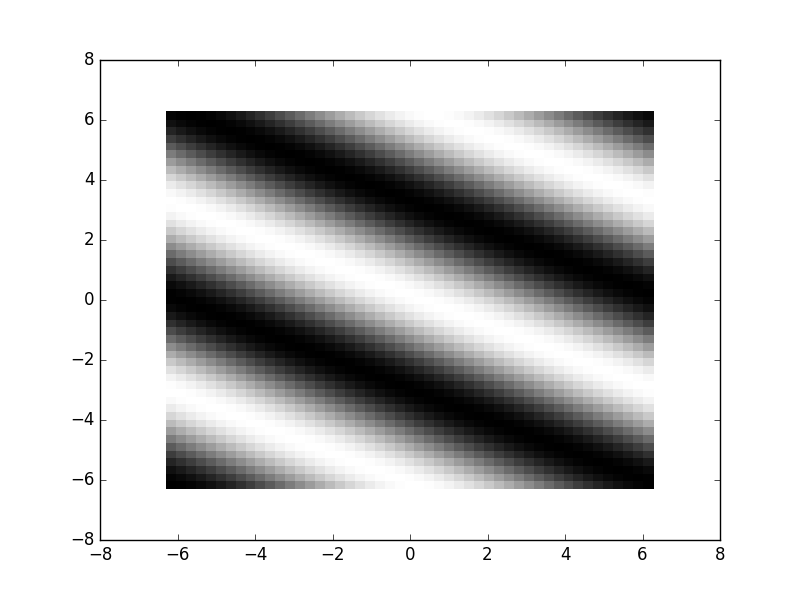
\includegraphics{sinusoidal1.png}
\end{figure}
\begin{figure}
    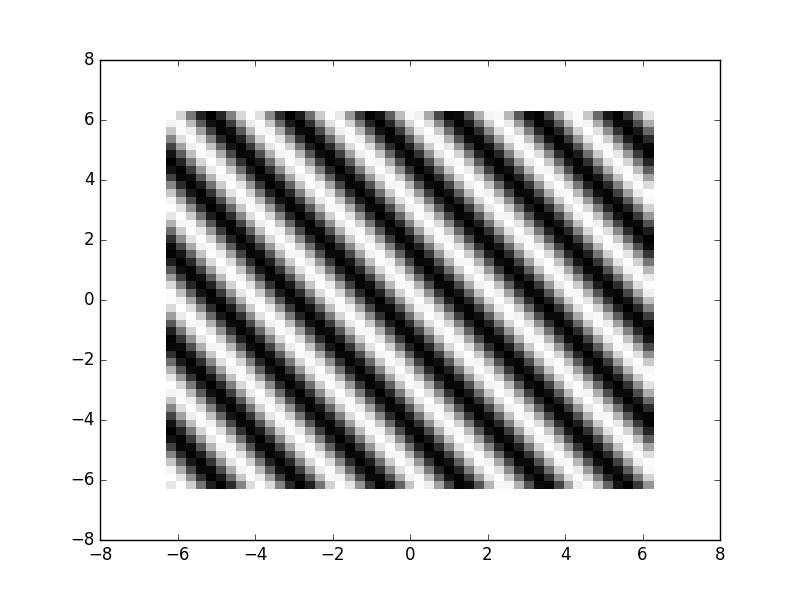
\includegraphics{sinusoidal2.png}
\end{figure}

The transformation from the spatial domain to the frequency domain can be done
using discrete Fourier transformation. The theory of discrete Fourier
transformation is quite involved and will not be reviewed here. The textbook
chapter 20 provides a mathematical treatment of the theory of Fourier analysis.
Details on how DFT is used for acquiring the frequency based representation are
provided in the textbook chapter 2.\cite{naturalimagestatistics} For now we are
going to focus on the uses of the frequency-based representation.

Linear filters and sinusoidals have a special relationship. The output of
linear filtering on a sinusoidal wave is a sinusoidal wave with same frequency
but possibly different phase and amplitude. If the input signal has the
following frequency-based representation
\begin{equation}
  I(x,y) = \sum_{\omega_{x}}{\sum_{\omega_{y}}{A_{\omega_{x},\omega_{y}}\cos(\omega_{x}x+\omega_{y}y+\Psi_{\omega_{x},\omega_{y}})}}
\end{equation}
the response of the linear filter has the following frequency-based representation
\begin{equation}
  O(x,y) = H(x,y) \ast I(x,y) = \sum_{\omega_{x}}{\sum_{\omega_{y}}{\lvert \tilde{H}(\omega_{x},\omega_{y})\rvert A_{\omega_{x},\omega_{y}} \cos(\omega_{x} x + \omega_{y} y + \Psi_{\omega_{x},\omega_{y}} + \angle\tilde{H}(\omega_{x},\omega_{y}))}}
\end{equation}
where $\lvert\tilde{H}(\omega_{x},\omega_{y})\rvert$ denotes the amplitude
magnification factor of the linear filter and
$\angle\tilde{H}(\omega_{x},\omega_{y})$ denotes the phase shift of the filter.
The $\lvert\tilde{H}(\omega_{x},\omega_{y})\rvert A_{\omega_{x},\omega_{y}}$
part of the equation is called the amplitude response.

Using this property of the frequency-based representation makes analysis of the
linear filters straightforward. It is difficult to describe the behavior of a
filter based solely on its spatial representation but if its amplitude response
is available you can tell what the filter does for different frequencies.

\subsubsection{Example of Linear Filtering}
\label{example-of-linear-filtering}
The concepts described above are demonstrated in the following code snippets.
In the first snippet a gaussian kernel is extracted from the SciPy gaussian
filtering operation using the properties of impulse response. NumPy is used
throughout the examples and the library name abbreviated as np.

\begin{lstlisting}[language=Python]
# Here we make use of the properties of the impulse response to get a gaussian
# kernel using the scipy gaussian filter. Create an array with all zeros except
# for one element in the center.
impulse = np.zeros((21,21))
impulse[10,10] = 1.

# Apply the gaussian filter to the impulse to obtain the gaussian kernel.
# gaussian_filter is scipy.ndimage.filters.gaussian_filter
gaussian_kernel = gaussian_filter(impulse, 3)
\end{lstlisting}
The gaussian kernel is shown in the following figure.
\begin{figure}
    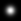
\includegraphics{kernel.png}
\end{figure}

In the second code snippet the filter is applied to an input image using 2d
convolution. The input image is just a 2d NumPy array containing the grayscale
input image. The image can be read using PIL, SciPy, OpenCV or similar.
\begin{lstlisting}[language=Python]
# Convolve the kernel with the example image
filtered_input = signal.convolve2d(img, gaussian_kernel)
\end{lstlisting}
The input image for the convolution is presented in the following figure. (source: \url{https://commons.wikimedia.org/wiki/File:Carl_Friedrich_Gauss_1840_by_Jensen.jpg})
\begin{figure}
    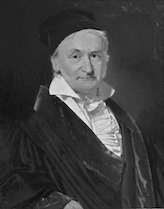
\includegraphics{input.png}
\end{figure}
And the corresponding output.
\begin{figure}
    
\includegraphics{output.png}
\end{figure}

In the last snippet the frequency-based representation of the gaussian kernel
is computed.
\begin{lstlisting}[language=Python]
# Compute the frequency-based representation of the filter
# fftshift is a convenience method for organizing the fft-output
f_b_representation = np.abs(np.fft.fftshift(np.fft.fft2(gaussian_kernel)))
\end{lstlisting}
The amplitude response of the filter kernel is shown below. In the picture dark
pixels correspond to small amplitude and light pixels correspond to high
amplitude. The amplitude of the 0 frequency is shown in the center of the
picture. The pixels away from the center have higher frequencies. The direction
where the pixel is from the center corresponds to the direction of the wave.
\begin{figure}
    
\includegraphics{freq.png}
\end{figure}
The gaussian filter does not have any surprising properties in the frequency
domain. In the frequency-based representation only the components very close to
the origin remain, which means the high-frequency components have been removed.
The final image is blurred as a result.

With a gaussian kernel computed with smaller standard deviation more of the
high frequency components are retained. The following figure presents the 
new kernel
\begin{figure}
    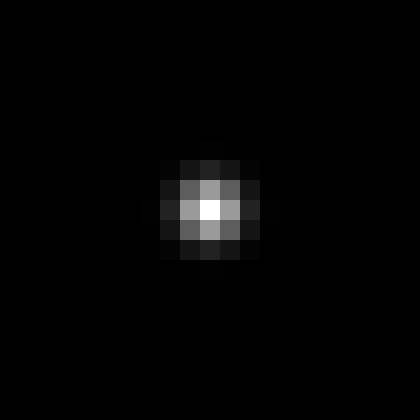
\includegraphics{kernel2.png}
\end{figure}
And the corresponding frequency-based representation shows that there are more
high frequency components retained.
\begin{figure}
    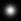
\includegraphics{freq2.png}
\end{figure}

\subsection{Frequency-based Representation as a Basis}
\label{frequency-based-representation-as-a-basis}
The frequency-based representation can be viewed as defining a basis and
finding coefficients in that basis. The idea is that any signal of the form $A
\cos(\omega x + \Psi)$ can be represented in the form $C\cos(\omega x) +
S\sin(\omega x)$ where S and C are some coefficients in our basis. This is
useful because defining S and C in a linear basis are linear operations and it
makes the calculation of amplitude $A$ and phase $\Psi$ simple. This rather
superficial treatment can be augmented by looking at the textbook section 2.3.
\begin{equation}
  A = \sqrt{C^{2}+S^{2}}
\end{equation}
\begin{equation}
  \Psi = -\arctan{\frac{S}{C}}
\end{equation}

\subsection{Space-frequency Analysis}
\label{space-frequency-analysis}
The tools described above are useful for analyzing linear filters but run into
trouble if we want to gain understanding about larger images. Running DFT on a
large image will give us a very high-level view on what sort of components the
image is made of, but it completely hides the spatial information in the
original image. Next we are going to look at methods that combine spatial and
frequential information.

Space-frequency analysis can be conducted by filtering the image with two
localized sinusoidal filters and computing the amplitudes of the filters. The
localized sinusoidal filters are called Gabor filters. On a high-level their
idea is that the sinusoidal plane wave is weighted by a windowing function,
making it very localized. The formula for coefficients C becomes
\begin{equation}
  C(x,y) = \sum_{x}{\sum_{y}{W(x-x_{0}, y-y_{0}) \cos(\omega_{x} (x - x_{0}) + \omega_{y} (y - y_{0})) }}
\end{equation}
The formula for coefficients S is similiar. With the coefficients C and S at
hand, the amplitudes can be calculated using the formula in the previous
section.

The windowing function $W(x,y)$ in the above formula for Gabor filters is the
Gaussian function. The width of the window can be controlled by changing the
$\sigma$ parameter of the Gaussian function. In 2d case there are separate
standard deviation parameters for both axes. In practical computation truncated
windows are used as the gaussian function falls off close to zero quickly.

\subsubsection{Example of Gabor Filtering}
\label{example-of-gabor-filtering}
In the following example Gabor filters are applied to an image to obtain a
spatial amplitude map of a vertical frequency component.

The input image.
\begin{figure}
    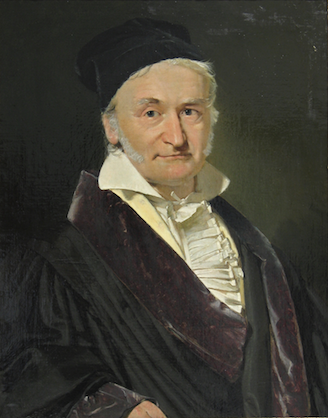
\includegraphics{input2.png}
\end{figure}

The gabor kernels, which are convolved with the input.
\begin{figure}
    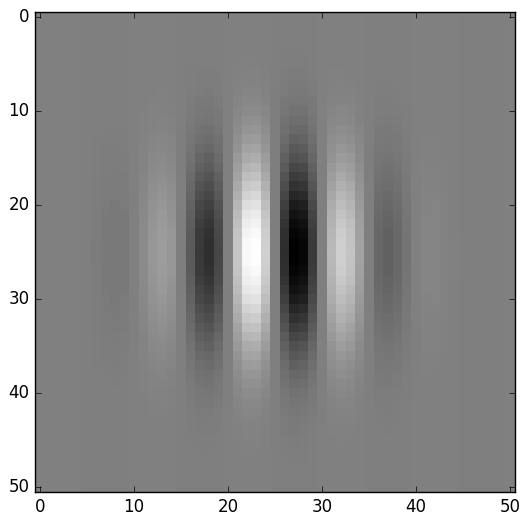
\includegraphics{gabor_kernel.png}
\end{figure}
\begin{figure}
    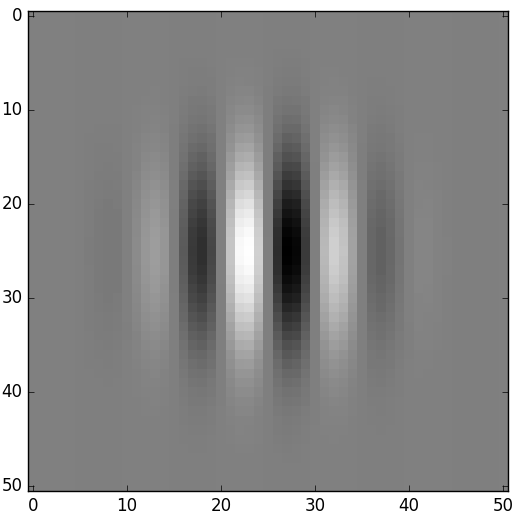
\includegraphics{gabor_kernel2.png}
\end{figure}

The spatial amplitude map. The amplitude is computed from the equation $A =
\sqrt{C^{2}+S^{2}}$.
\begin{figure}
    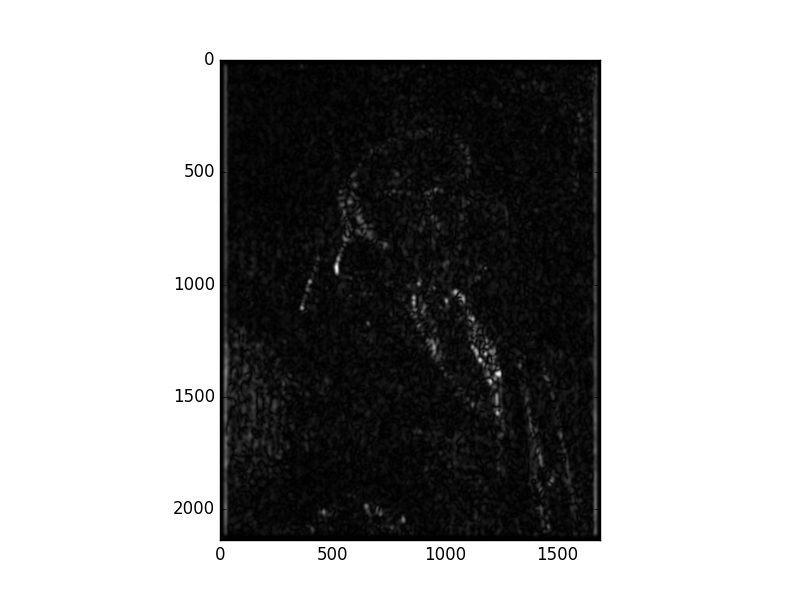
\includegraphics{gabor_output.png}
\end{figure}

\end{document}
